% VDE Template for EUSAR Papers
% Provided by Barbara Lang und Siegmar Lampe
% University of Bremen, January 2002
% English version by Jens Fischer
% German Aerospace Center (DLR), December 2005
% Additional modifications by Matthias Wei{\ss}
% FGAN, January 2009

%-----------------------------------------------------------------------------
% Type of publication
\documentclass[a4paper,10pt]{article}
%-----------------------------------------------------------------------------
% Other packets: Most packets may be downloaded from www.dante.de and
% "tcilatex.tex" can be found at (December 2005):
% http://www.mackichan.com/techtalk/v30/UsingFloat.htm
% Not all packets are necessarily needed:
\usepackage[T1]{fontenc}
\usepackage[latin1]{inputenc}
%\usepackage{ngerman} % in german language if required
\usepackage[nooneline,bf]{caption} % Figure descriptions from left margin
\usepackage{times}
\usepackage{multicol}
\usepackage{amsmath}
\usepackage{amssymb}
\usepackage[dvips]{graphicx}
\usepackage{epsfig}
\input{tcilatex}
%-----------------------------------------------------------------------------
% Page Setup
\textheight24cm \textwidth17cm \columnsep6mm
\oddsidemargin-5mm                 % depending on print drivers!
\evensidemargin-5mm                % required margin size: 2cm
\headheight0cm \headsep0cm \topmargin0cm \parindent0cm
\pagestyle{empty}                  % delete footer and header
%----------------------------------------------------------------------------
% Environment definitions
\newenvironment*{mytitle}{\begin{LARGE}\bf}{\end{LARGE}\\}%
\newenvironment*{mysubtitle}{\bf}{\\[1.5ex]}%
\newenvironment*{myabstract}{\begin{Large}\bf}{\end{Large}\\[2.5ex]}%
%-----------------------------------------------------------------------------
% Using Pictures and tables:
% - Instead "table" write "tablehere" without parameters
% - Instead "figure" write "figurehere " without parameters
% - Please insert a blank line before and after \begin{figuerhere} ... \end{figurehere}
%
% CAUTION:   The first reference to a figure/table in the text should be formatted fat.
%
\makeatletter
\newenvironment{tablehere}{\def\@captype{table}}{}
\newenvironment{figurehere}{\def\@captype{figure}\vspace{2ex}}{\vspace{2ex}}
\makeatother



%%%%%%%%%%%%%%%%%%%%%%%%%%%%%%%%%%%%%%%%%%%%%%%%%%%%%%%%%%%%%%%%%%%%%%%%%%%%%%
\begin{document}

% Please use capital letters in the beginning of important words as for example
\begin{mytitle}Pedometer for STM32F4\end{mytitle}
\begin{mysubtitle}Use the MEMS accelerometer to count number of steps\end{mysubtitle}
%
% Please do not insert a line here
%
\\
De Donatis Emanuele\\
Matr. 817667, (emanuele.dedonatis@mail.polimi.it)\\
\hspace{10ex}
Pistone Bruno\\
Matr. 818949, (bruno.pistone@mail.polimi.it)\\
\begin{flushright}
\emph{Report for the master course of Embedded Systems}\\
\emph{Reviser: PhD. Patrick Bellasi (bellasi@elet.polimi.it)}
\end{flushright}

Received: November, 04 2013\\
\hspace{10ex}

\begin{myabstract} Abstract \end{myabstract}
This project is part of a collaborative project whose purpose is to develop a simple 
yet realistic training support system. The goal of this project is to develop a pedometer 
using the MEMS motion sensor on the STM32F4DISCOVERY board. The device provides
the user with statistics about its training activity.

\vspace{4ex}	% Please do not remove or reduce this space here.
\begin{multicols}{2}

%%%%%%%%%%%%%%%%%%%%%%%%%%%%%%%%%%%%%%%%%%%%%%%%%%%%%%%%%%%%%%%%%%%%%%%%%%%%%
\section{Introduction}
During the Real-Time Operating System course of the Polytechnic of Milan has been
proposed a collaborative project whose aim is to develop a Personal Trainer device
based on the economical development board STM32F4DISCOVERY and the 
Miosix embedded OS. 

Each group was assigned one of the following modules:
{\small
\begin{center}
\begin{tabular}{|l|c|r|} \hline
{\bf Module Name} & {\bf Device}\\ \hline
Pedometer & MEMS \\
User Interface & UART, Flash\\
Audio Feedback & CS43L22 (DAC) \\
Voice Commands & NONE (PCM Samples) \\
PCM Encoding & MP45DT02 MEMS Mic\\
Social Wireless & NRF24L01 2.4GHz TxRx\\
Context Awareness & ADC \\ \hline
\end{tabular}
\end{center}
}

The final goal is to join each module in order to build a working system.

%-----------------------------------------------------------------------------
\subsection{STM32F4DISCOVERY board}
% Please avoid separations in titles
% and separate text manually

The STM32F4DISCOVERY is an evaluation board by STMicroelectronics, based on the ARM Cortex-M4F core.

{\small
\begin{itemize}
\item STM32F407VGT6 microcontroller featuring 32-bit ARM Cortex-M4F core, 1 MB Flash, 192 KB RAM in an LQFP100 package
\item LIS302DL or LIS3DSH ST MEMS 3-axis accelerometer
\item MP45DT02, ST MEMS audio sensor, omni-directional digital microphone
\item CS43L22, audio DAC with integrated class D speaker driver
\item USB OTG FS with micro-AB connector
\end{itemize}
}
\begin{figurehere}
 \centering
 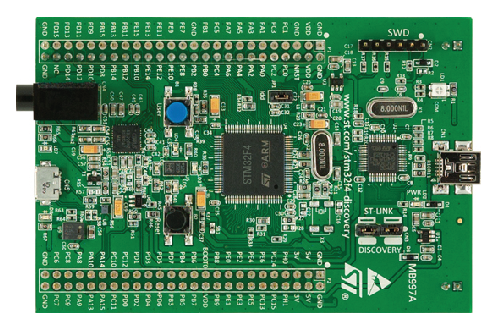
\includegraphics[width=8cm, height=5cm]{./eps/STM32F4.eps}
 \caption{STM32F4DISCOVERY board}
 \label{fig:STM32F4}
\end{figurehere}

%-----------------------------------------------------------------------------
\subsection{MIOSIX embedded OS}
% Please avoid separations in titles
% and separate text manually

Miosix is a kernel designed to run on 32bit microcontrollers, in active development since 2008.

It is designed as a single process, multiple threads kernel, that matches the capabilities of microcontrollers (i.e., the lack of an MMU). Applications are statically linked with the kernel and standard library forming one binary file suitable to be loaded onto a microcontroller.

Miosix is designed in a way to hide the boot process from the user. When main() is called, the kernel has already started. Indeed, main() itself is a thread. To achieve this result the initialization of the basic hardware functionalities required for the kernel to boot is coded in a board support package.

The kernel is licensed under the GPL license with an exception that allows it to be linked with propietary application code.

%-----------------------------------------------------------------------------
\subsection{MEMS Motion Sensor}
% Please avoid separations in titles
% and separate text manually

The STM32F4DISCOVERY includes the LIS302DL ST MEMS motion sensor.
It is an ultra compact low-power three-axis linear accelerometer. It includes
a sensing element and an IC interface able to provide the measured acceleration
to the external world through I2C/SPI serial interface.

The STM32F4 controls this motion sensor through the SPI interface (see {\bf Figure
\ref{fig:LIS302DL}}). 

\begin{figurehere}
 \centering
 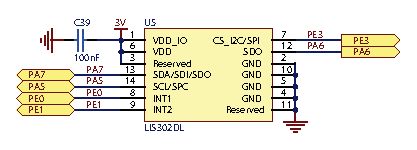
\includegraphics[width=8cm, height=3cm]{./eps/LIS302DL.eps}
 \caption{LIS302DL Motion Sensor}
 \label{fig:LIS302DL}
\end{figurehere}

%%%%%%%%%%%%%%%%%%%%%%%%%%%%%%%%%%%%%%%%%%%%%%%%%%%%%%%%%%%%%%%%%%%%%%%%%%%%%
\section{Pedometer Algorithm}

To develop the pedometer algorithm we relied on the Neil Zhao's model .\cite{NeilZhao}


%-----------------------------------------------------------------------------
\subsection{Digital Filter}

First, a digital filter is needed to smooth the signals. Four registers and a summing unit can be used  (see {\bf Figure
\ref{fig:DigitalFilter}}).  Of course, more registers could be used to make the acceleration data smoother, but the response time would be slower.

\begin{figurehere}
 \centering
 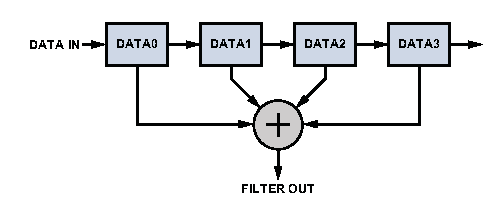
\includegraphics[width=7cm, height=3cm]{./eps/DigitalFilter.eps}
 \caption{Digital filter}
 \label{fig:DigitalFilter}
\end{figurehere}

%-----------------------------------------------------------------------------
\subsection{Dynamic Threshold and Dynamic Precision}

The system continuously updates the maximum and minimum values of the 3-axis acceleration every 50 samples. The average value, (Max + Min)/2, is called the dynamic threshold level. 

\begin{figurehere}
 \centering
 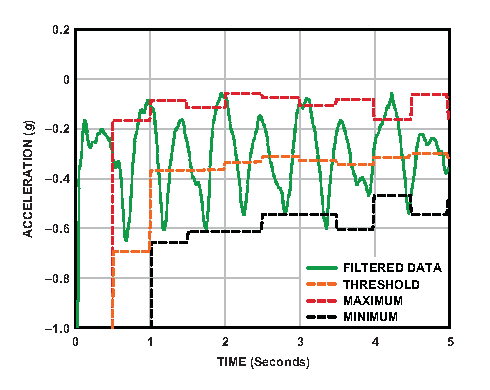
\includegraphics[width=8cm, height=5cm]{./eps/Threshold.eps}
 \caption{Acceleration curves}
 \label{fig:Threshold}
\end{figurehere}

For each axis two registers, sample\textunderscore new and sample\textunderscore old, are used to pick out new sample result. When a new data sample comes, sample\textunderscore new is shifted to the sample\textunderscore old register unconditionally. However the new sample result will be shifted into the sample\textunderscore new register only if the changes in acceleration are greater than a predefined precision; otherwise the sample\textunderscore new register will remain unchanged. The shift register group can thus remove the high-frequency noise and make the decision more precise.

\begin{figurehere}
 \centering
 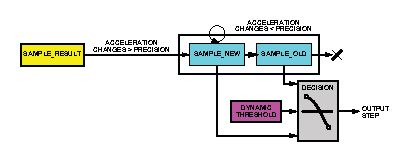
\includegraphics[width=8cm, height=3cm]{./eps/RegistersDiagram.eps}
 \caption{Dynamic threshold and dynamic precision}
 \label{fig:RegistersDiagram}
\end{figurehere}

%-----------------------------------------------------------------------------
\subsection{Step}

A step is defined as happening if there is a negative slope of the acceleration plot (sample\textunderscore new < sample\textunderscore old) when the vertical acceleration curve crosses below the dynamic threshold.

The vertical axis is the one with the greatest threshold level since it reads also the gravitational acceleration.

%-----------------------------------------------------------------------------
% We suggest the use of JabRef for editing your bibliography file (Report.bib)
\bibliographystyle{splncs}
\bibliography{Report}

\end{multicols}
\end{document}
